\documentclass[serif]{beamer}
%\usepackage[utopia]{mathdesign}
%\usepackage[no-math]{fontspec}
%\setmainfont{Liberation Serif}

\usepackage{minted}
% \usepackage{redhat}
\usepackage{hyperref}
\usepackage{ccicons}
\usepackage{ulem}
\usepackage{changepage}

% \usepackage{tikz}
% \usetikzlibrary{arrows,shapes,snakes,automata,backgrounds,petri}

%gets rid of bottom navigation bars
\setbeamertemplate{footline}[page number]{}

%gets rid of navigation symbols
\setbeamertemplate{navigation symbols}{}

\title{Brave new world of unified cgroups}
\author{Michal Sekletár\\Zbigniew Jędrzejewski-Szmek}
\institute{%
  
\includegraphics[width=10em]{images/Logo-redhat-color-375.png}\\
  \medskip
  \textit{msekleta@redhat.com\\zbyszek@in.waw.pl}\\
  \medskip
  \ccbysa
}
\date{\tiny Brno, 2020.01.24}

\begin{document}
\begin{frame}
\titlepage % Print the title page as the first slide
\end{frame}

\begin{frame}
  \frametitle{Why this talk?}
  \pause

  Unified hierarchy (a.k.a.) cgroups v2 is the default default in systemd 243 (Sept.\ 2019)\\[1em]
  \url{https://fedoraproject.org/wiki/Changes/CGroupsV2} (for F31+)\\[1em]
  Version two is just nicer!
\end{frame}

\begin{frame}
  \frametitle{Control groups}

  Control groups (cgroups) is a Linux subsystem that has two main purposes:
  \begin{itemize}
  \item Process tracking
  \item Resource distribution
  \end{itemize}
\end{frame}

\begin{frame}
  \frametitle{Control groups}

  \textbf{Cgroup} – associates a set of tasks with a set of parameters for one or
  more controllers\\

  \textbf{Controller} – schedules a resource or applie per-cgroup limits\\

  \textbf{Hierarchy} – set of cgroups arranged in a tree, every process
  is in exactly one cgroup
\end{frame}

\begin{frame}
  \frametitle{Brief history of cgroups in the linux kernel}

  \begin{adjustwidth}{-1.5em}{-1.5em}
    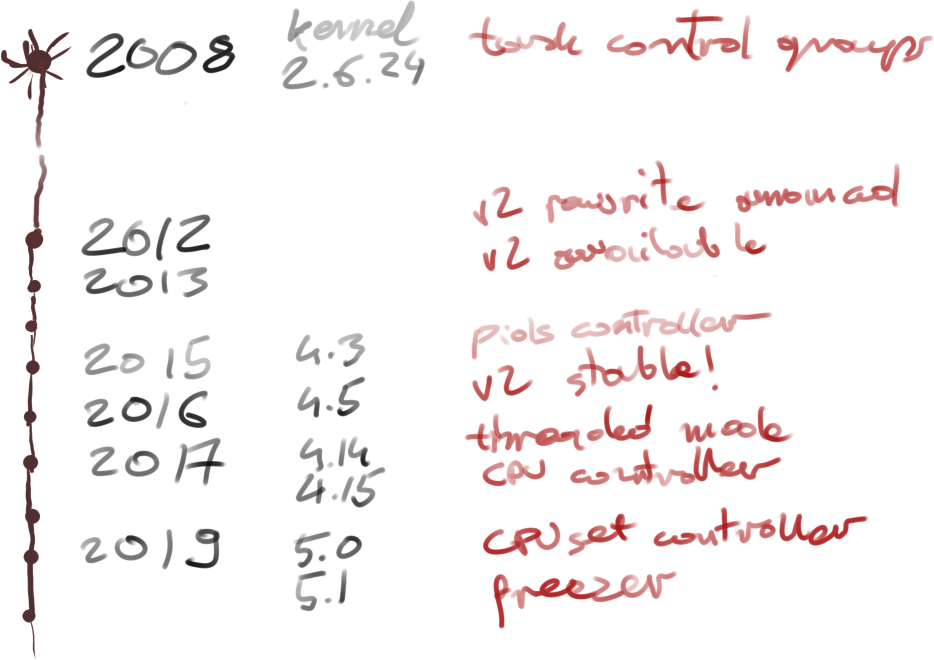
\includegraphics[width=\textwidth]{images/cgroup-history.png}
  \end{adjustwidth}
\end{frame}

\begin{frame}
  \frametitle{Why?}

\end{frame}

\begin{frame}
  \frametitle{What's wrong with v1}

  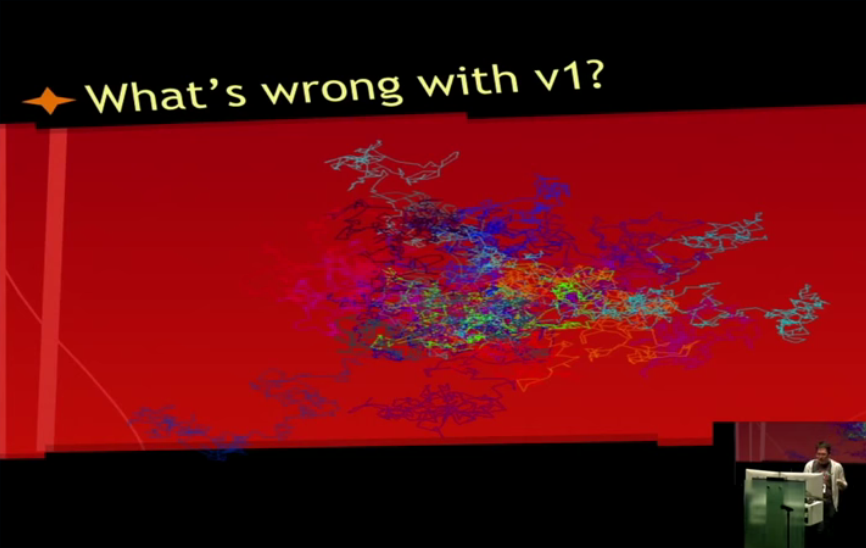
\includegraphics[width=\textwidth]{images/whats-wrong.png}
\end{frame}

\begin{frame}
  \frametitle{What's wrong with v1}

  \begin{itemize}
  \item design follows implementation \pause
  \item inconsistent interface \pause
  \item infinite number of hierarchies \pause
  \item not hierarchical \pause
  \item unusable limits \pause
  \item no cooperation between contollers\pause
  \item threads not processes \pause
  \item no secure delegation
  \end{itemize}
\end{frame}

\begin{frame}[fragile]
\begin{adjustwidth}{-1.5em}{-1.5em}
\begin{minted}{console}
$ ls /sys/fs/cgroup/memory/
...
memory.limit_in_bytes       memory.kmem.tcp.limit_in_bytes
memory.usage_in_bytes       memory.kmem.tcp.usage_in_bytes
memory.max_usage_in_bytes   memory.kmem.tcp.max_usage_in_bytes
memory.soft_limit_in_bytes

memory.kmem.limit_in_bytes     memory.memsw.limit_in_bytes
memory.kmem.usage_in_bytes     memory.memsw.usage_in_bytes
memory.kmem.max_usage_in_bytes memory.memsw.max_usage_in_bytes

memory.kmem.slabinfo             memory.use_hierarchy
memory.move_charge_at_immigrate  cgroup.sane_behavior
...
\end{minted}
\end{adjustwidth}
\end{frame}

\begin{frame}[fragile]
  \frametitle{inconsistent interface}

  \begin{tabular}{l|rr}
    v1                        & default & range           \\
    \texttt{cpu.shares}       & 1024 & 2-262144 \\
    \texttt{blkio.bfq.weight} & 500  & 10–1000 \\
    \hline
    v2           \\
    \texttt{cpu.weight}       & 100  & 1–10000 \\
    \texttt{io.weight}%
    \footnote{\textcolor{gray}{\url{https://github.com/systemd/systemd/pull/13335}}}
    & 100  & 1–10000
  \end{tabular}
\end{frame}

\begin{frame}
  \frametitle{v2}

  Design:
  \begin{itemize}
  \item single hierarchy
  \item consistent interface
  \item small number of controllers: memory, io, pids, cpu, cpuset
  \item controllers are fully hierarchical
  \item (controllers can be turned off midway throught the tree)
  \item high-level knobs
  \item soft limits
  \item non-hierarchical controllers are gone
  \end{itemize}
\end{frame}

\begin{frame}[fragile]
  \frametitle{Old vs. New}

  \begin{tabular}{l|l}
    v1 controller          &  v2 solution\\
    \hline
    memory                 &  memory \\
    cpu+cpuacct            &  cpu    \\
    cpuset                 &  cpuset \\
    blkio                  &  io     \\
    pids                   &  pids   \\
    hugetlb                &  hugetlb (kernel 5.6)\\[1em]\pause

    freezer                &  replaced by cgroup.freeze\\[1em]\pause
    devices                &  eBPF filters \\[1em]\pause
    net\_cls,net\_prio     &  matching by cgroup, eBPF\\
    perf\_event            &  eBPF
  \end{tabular}
\end{frame}




\setbeamercolor{background canvas}{bg=yellow}

\begin{frame}
  \frametitle{Delegation}

  \begin{itemize}
  \item less-privileged process owns a part of the cgroup tree
  \item implemented through file system permissions
  \item Delegate=yes in systemd units
  \item cutoff \emph{not} at the directory level
  \end{itemize}
\end{frame}

\begin{frame}[fragile]
  \tiny
  \frametitle{\texttt{\$ sudo systemd-cgls}}
  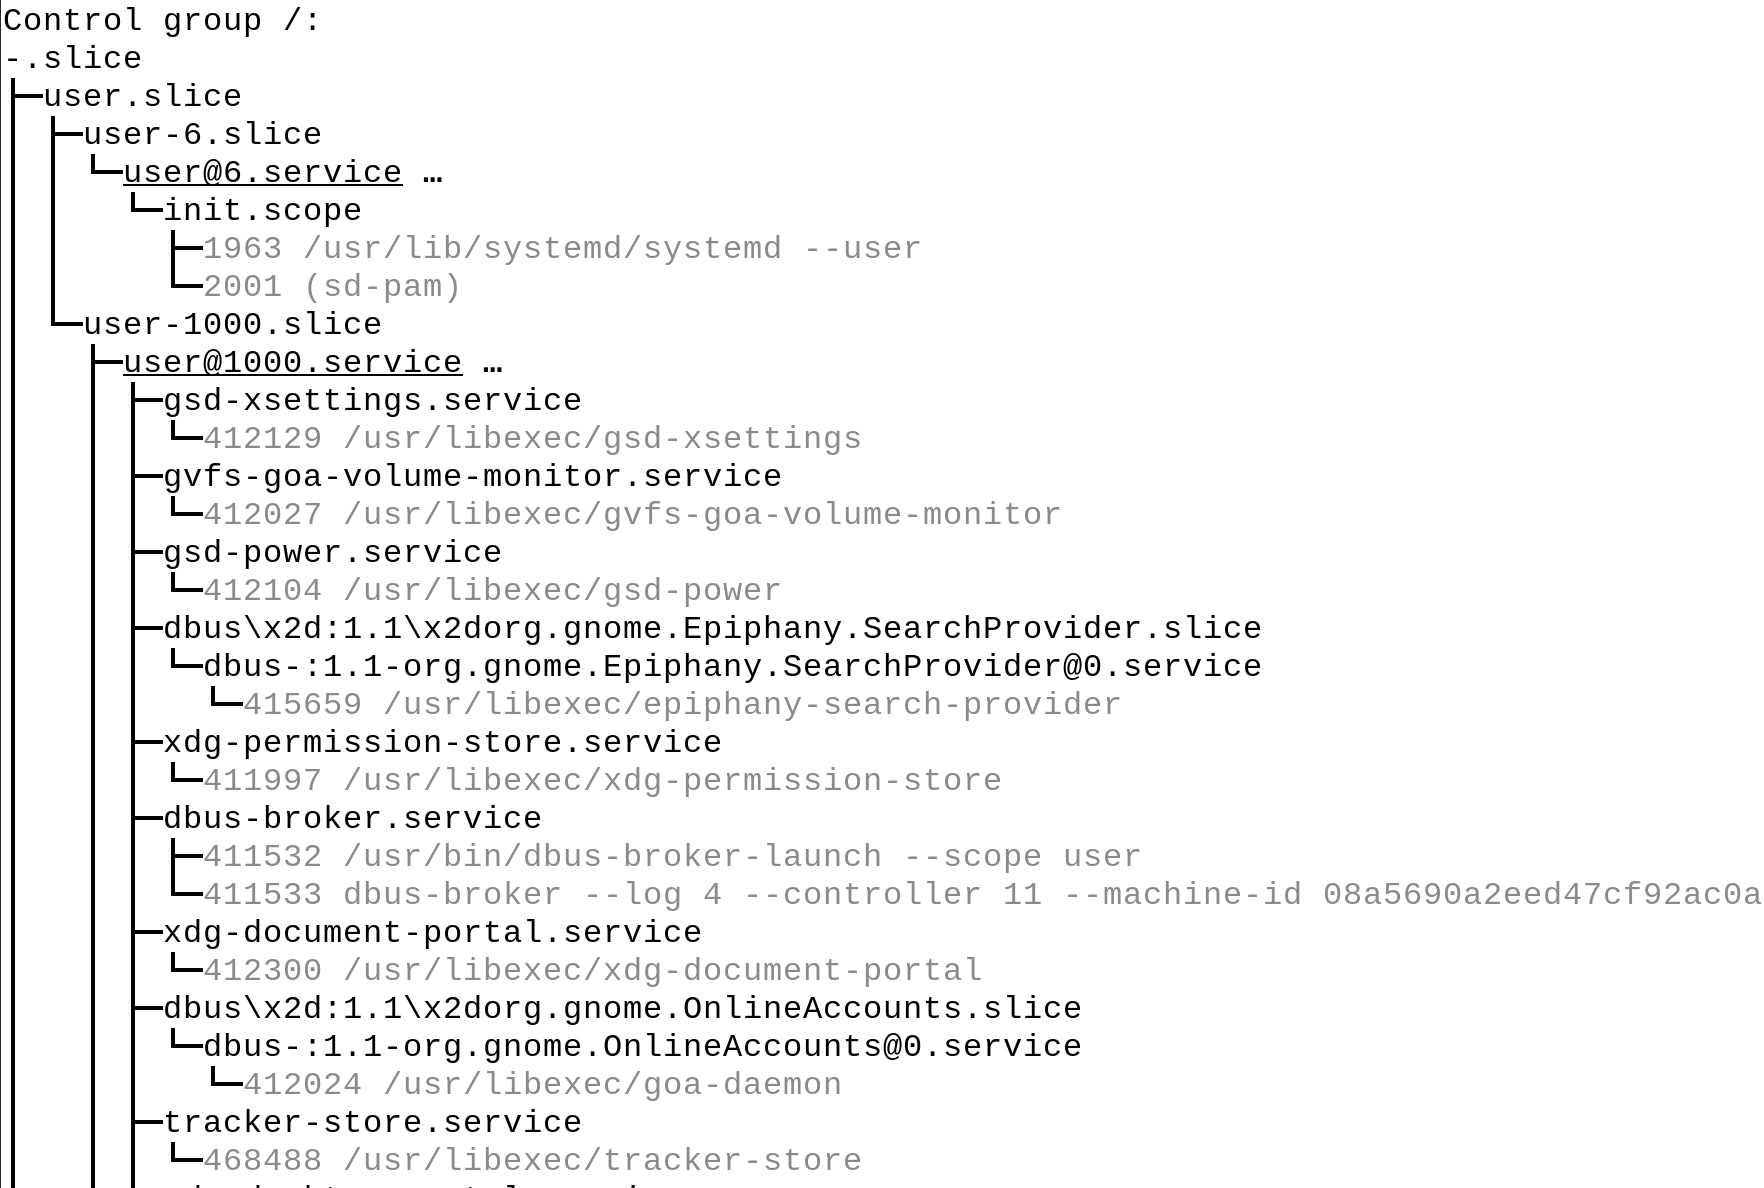
\includegraphics[width=\textwidth]{images/delegation-cgls.png}
\end{frame}

\begin{frame}[fragile]
  \begin{minted}{console}
$ ls -l .../user.slice/user-1000.slice/user@1000.service
-r--r--r--. root    root    cgroup.controllers
-r--r--r--. root    root    cgroup.events
-rw-r--r--. root    root    cgroup.freeze
-rw-r--r--. root    root    cgroup.max.depth
-rw-r--r--. root    root    cgroup.max.descendants
-r--r--r--. root    root    cgroup.stat
-rw-r--r--. zbyszek zbyszek cgroup.procs
-rw-r--r--. zbyszek zbyszek cgroup.threads
-rw-r--r--. zbyszek zbyszek cgroup.subtree_control
-r--r--r--. root    root    pids.current
-r--r--r--. root    root    pids.events
-rw-r--r--. root    root    pids.max
...
drwxr-xr-x. zbyszek zbyszek pipewire.service/
drwxr-xr-x. zbyszek zbyszek pulseaudio.service/
drwxr-xr-x. zbyszek zbyszek xdg-desktop-portal-gtk.service/
drwxr-xr-x. zbyszek zbyszek xdg-desktop-portal.service/
drwxr-xr-x. zbyszek zbyszek xdg-document-portal.service/
  \end{minted}
\end{frame}

\begin{frame}
  \frametitle{Delegation}
  \framesubtitle{is not all or nothing}

  \begin{itemize}
  \item Delegate=io pids memory ...
  \item delegation may be nested
  \item resources are divided hierarchically
  \end{itemize}
\end{frame}

\setbeamercolor{background canvas}{bg=green}

\begin{frame}[fragile]
  \frametitle{Threaded mode}

  \pause

  v1 operated on threads, v2 operates on processes
  \medskip\pause

  only supported by selected controllers (cpu, cpuset)
  \medskip\pause

  a leaf cgroup may be switched to threaded mode and subdivided\\
  \mintinline{console}{        $ echo threaded > $CGROUP/cgroup.type}\\
  \pause

  \texttt{cgroup.threads}
  \medskip\pause

  used by libvirt
\end{frame}

\setbeamercolor{background canvas}{bg=orange}

\begin{frame}
  \frametitle{Resource management\,--\,Resource distribution models}

  \begin{itemize}
  \item \textbf{Weights}
    \begin{itemize}
    \item Resource is distributed by adding up the weights of all sub-cgroups and giving each the fraction matching its ratio against the sum.
    \item Usually used to distribute stateless resources (CPU time)
    \item Example: cpu.weight ([1-10000], default 100)
    \end{itemize}
    \pause

  \item \textbf{Limits}
    \begin{itemize}
    \item Cgroup can consume up to configured amount of the resource
    \item Overcommit is allowed (i.e. sum of sub-cgroup limits can exceed limit of the parent cgroup)
    \item Example: memory.max
    \end{itemize}
    \pause

  \item \textbf{Protections}
    \begin{itemize}
    \item Cgroup is protected (but not guaranteed) up to configured amount of the resource
    \item Overcommit is also allowed
    \item Example: memory.low
    \end{itemize}
    \pause

  \item \textbf{Allocations}
    \begin{itemize}
    \item Exclusive allocations of the absolute amount of a finite resource (e.g. real-time budget)
    \end{itemize}
  \end{itemize}
\end{frame}

\begin{frame}
  \frametitle{Memory protections and limits}

  \begin{adjustwidth}{-2em}{-2em}
    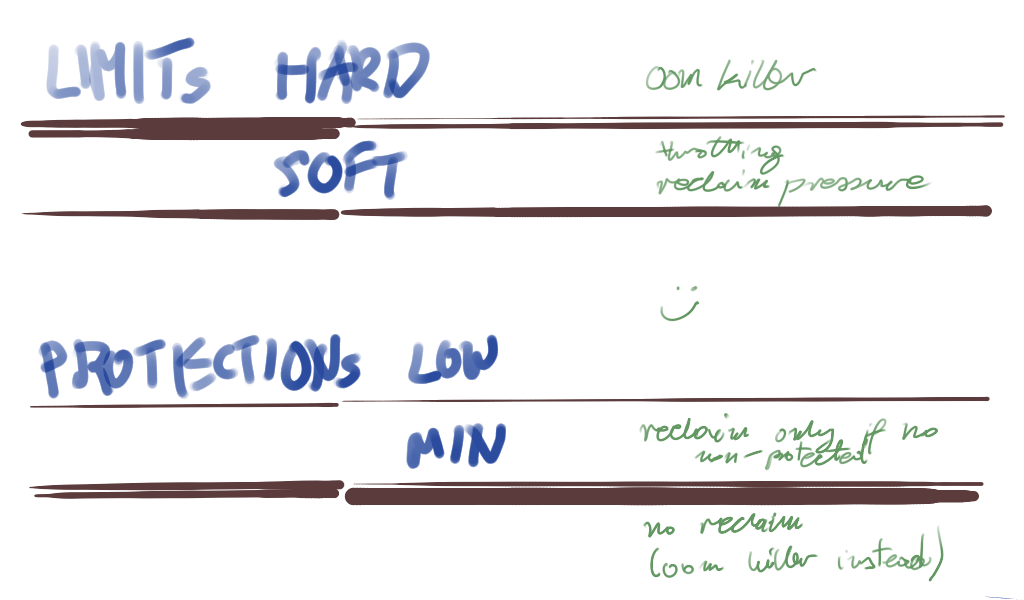
\includegraphics[width=\paperwidth]{images/memory-protection.png}
  \end{adjustwidth}
\end{frame}

\begin{frame}
  \frametitle{Resource management\,--\,Memory}
  Partitioning available memory with systemd and cgroup v2 memory controller is rather complicated. Multiple options are available,
  \begin{itemize}
  \item \textbf{memory.min}\,--\,Hard memory protection. If memory usage is below the limit the cg memory won't be reclaimed.
  \item \textbf{memory.low}\,--\,Soft memory protection. If memory usage is below the limit the cg memory can be reclaimed only if there is no memory to be reclaimed from unprotected cgroups.
  \item \textbf{memory.high}\,--\,Memory throttle limit. If memory usage goes above the limit the processes in the cgroup are throttled and put under heavy reclaim pressure.
  \item \textbf{memory.max}\,--\,Hard limit for memory usage. You can use K, M, G, T suffixes (e.g. MemoryMax=1G).
  \end{itemize}

  After you exhaust your memory limit then service is very likely to
  get killed by OOM killer. To prevent that you need to adjust
  \texttt{OOMScoreAdjust} value as well.
\end{frame}

\begin{frame}
  \frametitle{Resource management\,--\,Block I/O}
  \texttt{io} controller in cgroup v2 allows for quite fine grained tuning.
  systemd provides following options for configuring this subsystem:
  \begin{itemize}
  \item \textbf{io.weight}\,--\,IO weight
  \item \textbf{io.max}\,--\,per-device absolute bandwidth limit (e.g. \texttt{8:16 rbps=2097152 wiops=120})
  \item \textbf{io.latency}\,--\,per-device latency target protection (e.g. \texttt{8:16 target=10000})
  \end{itemize}
\end{frame}

\begin{frame}


\end{frame}

\setbeamercolor{background canvas}{bg=cyan}

\begin{frame}
  \frametitle{Status quo}

  v1 only: k8s, CRI-O, Docker, Containerd, runc (in progress), OCI runtime spec

  \medskip

  v2 too: Buildah+Podman+skopeo, crun, libvirt, JVM, snapd, systemd
\end{frame}

%% \begin{frame}
%%   \frametitle{What is happening now?}

%%   CPUSET in kernel 5.0, freezer in kernel 5.1\\\pause
%%   (systemd supports both and translates v2 settings for v1)\\\pause
%%   https://fedoraproject.org/wiki/Changes/CGroupsV2\\\pause
%%   JVM, libvirt, snapd patched\\\pause
%%   crun works\\
%%   docker/mobi and most container runtimes — nope\\\pause
%%   ``Red Hat suite'': podman, buildah, skopeo — works
%% \end{frame}

\begin{frame}
  \frametitle{Status of container runtimes}

  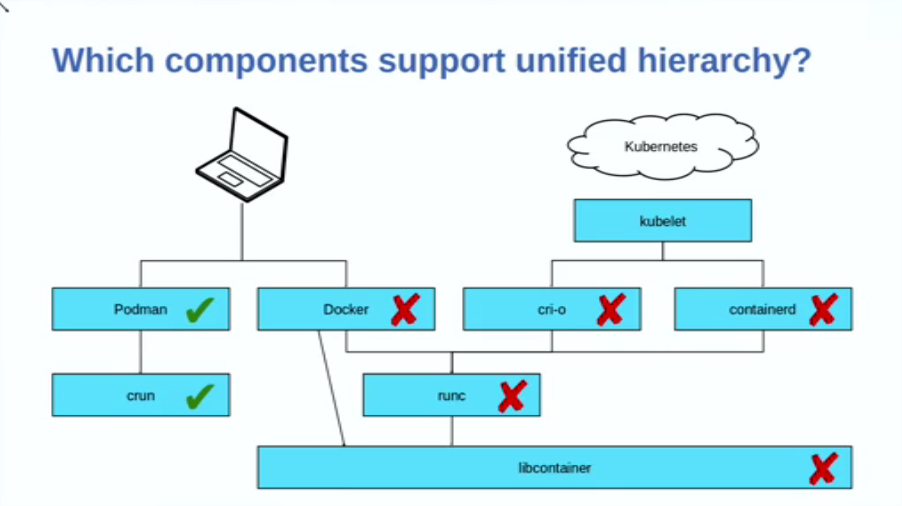
\includegraphics[width=\textwidth]{images/container-runtime-status.png}
\end{frame}


\setbeamercolor{background canvas}{bg=white}

\begin{frame}
  \frametitle{Summary}

  control groups v2:
  \begin{itemize}
  \item fully hierarchical with safe delegation
  \item consistent inteface
  \item efficient and scalable notifications
  \item fewer controllers, high-level knobs
  \item soft limits
  \item eBPF!
  \item better monitoring: PSI!
  \end{itemize}
\end{frame}






\begin{frame}[fragile]
  \frametitle{Links}
  \tiny

  this talk: \url{https://github.com/keszybz/cgroupsv2/raw/master/cgroupsv2.pdf}

  \medskip

  docs:\\
  \url{https://www.kernel.org/doc/html/latest/admin-guide/cgroup-v1/}\\
  \url{https://www.kernel.org/doc/html/latest/admin-guide/cgroup-v2.html}\\
  \url{https://facebookmicrosites.github.io/cgroup2/docs/overview}\\
  \href{https://www.freedesktop.org/software/systemd/man/systemd.resource-control.html}{systemd.resource-control(5)}\\
  \url{https://systemd.io/CGROUP_DELEGATION.html}

  \medskip

  recent changes: \\
  \url{https://www.redhat.com/sysadmin/fedora-31-control-group-v2}\\
  \url{https://fedoraproject.org/wiki/Changes/CGroupsV2}\\
  \url{https://www.youtube.com/watch?v=GznkuTXq8AQ&t=1s}\\
  \url{https://medium.com/nttlabs/cgroup-v2-596d035be4d7}\\
  \url{https://www.youtube.com/watch?v=yZpNsDe4Qzg} (Michael Kerrisk)

  freezer for cgroup v2 \href{https://git.kernel.org/pub/scm/linux/kernel/git/torvalds/linux.git/commit/v5.1-rc3-45-g76f969e894}{v5.1-rc3-45-g76f969e894}\\
  \url{https://lwn.net/Articles/772377/}

  \url{https://bugzilla.redhat.com/show_bug.cgi?id=1727149} libvirt support in 5.5.0
  \url{https://bugzilla.redhat.com/show_bug.cgi?id=1438079} snapd support in snapd-2.41-1.fc31
  \url{https://github.com/opencontainers/runc/pull/2113} for libcontainer
  \url{https://github.com/opencontainers/runc/issues/654} for runc
  \url{https://github.com/kubernetes/enhancements/pull/1370/files} for k8s
  \href{https://codesearch.debian.net/search?q=cgroup.type&literal=1&perpkg=1}{codesearch.debian.net/search?q=cgroup.type}
  \url{https://www.kernel.org/doc/html/latest/accounting/psi.html}
\end{frame}

\begin{frame}[fragile]
  \frametitle{Links}
  \tiny

  history:\\
  \url{https://kernelnewbies.org/Linux_2_6_24#Task_Control_Groups}

  \url{https://kernelnewbies.org/Linux_3.16#Unified_Control_Group_hierarchy}

  \href{https://lwn.net/Articles/697369/}{State of CPU controller in cgroup v2} (2016)

  \href{https://lwn.net/Articles/729215/}{LWN: A milestone for control groups} (2017)

  \href{https://kernelnewbies.org/Linux_4.15#Better_CPU_usage_restrictions_with_the_CPU_resource_controller_for_cgroupv2}{Linux 4.15}

  \href{https://git.kernel.org/pub/scm/linux/kernel/git/torvalds/linux.git/commit/?id=v4.14-rc2-7-g0d5936344f}{v4.14-rc2-7-g0d5936344f}

  \url{https://www.youtube.com/watch?v=PzpG40WiEfM}

  \url{https://www.youtube.com/watch?v=ikZ8_mRotT4}
\end{frame}

\end{document}
